\vspace{-2em}
\section{Inductive Analysis}

Recursion employs techniques of repeatedly shrinking the problem to solve its smaller halves. Often found in sorting problems, processing trees, and
geometric problems.

\begin{theo}[MergeSort]
    
    Given an array $A$ of size $n$, we sort via the following:
    \begin{enumerate}
        \item [(i.)] Recursively: Split the array into two halves and wait for a return.
        \item [(ii.)] Base-case: If the array has one element, return it.
        \item [(iii.)] Merge: receive two halves and merge them.
    \end{enumerate}
    The final result is a sorted array.
\end{theo}

\begin{theo}[QuickSort]

    Given an array $A$ of size $n$, we sort via the following:
    \begin{enumerate}
        \item [(i.)] Choose a pivot, set $i$ to the start and $j$ at the end of the array.
        \item [(ii.)] Increase $i$ until $A[i]>pivot$ and decrease $j$ until $A[j]<pivot$.
        \begin{itemize}
            \item If $A[i]<A[j]$, swap $A[i]$ and $A[j]$.
            \item Repeat until $i>j$, return $j$ as the new pivot.
        \end{itemize}
        \item [(iii.)] The new pivot creates two sub-arrays, repeat the process on each sub-array.
    \end{enumerate}
    The final result is $A$ sorted in-place (on the original array without a temporary helper array).
\end{theo}

\begin{Tip} Demos for 
 \textbf{MergeSort}: \url{https://www.youtube.com/watch?v=4VqmGXwpLqc} and\\
 \textbf{QuickSort}: \url{https://www.youtube.com/watch?v=Hoixgm4-P4M}.
\end{Tip}

\newpage

\begin{Func}[Mergesort - \texttt{MSORT(A)}]
    \textbf{Input:} Array $A$ and temporary array $temp$ of $n$ elements.\\
    \textbf{Output:} Nothing is returned, the array $A$ is sorted by reference.\\

    \vspace{-.5em}
    \noindent
    \textbf{MSORT function:}\\
    \begin{algorithm}[H]
        \label{algo:mergesort}
        \If{$i \geq j$}{
            \Return;
        }
            $mid \gets (i + j) / 2$\;
            $MSORT(A, temp, i, mid);$ \tcp{Left subarray}
            $MSORT(A, temp, mid + 1, j);$ \tcp{Right subarray}
            $merge(A, temp, i, mid, mid + 1, j);$ \tcp{Merge both halves}
        
    \end{algorithm}

    \vspace{.5em}

    \noindent
    \textbf{Merge function:}\\
    \begin{algorithm}[H]
        $i \gets lefti$; \tcp{Left subarray}
        $j \gets righti$; \tcp{Right subarray}
        $k \gets lefti$; \tcp{Temporary array}
        
        \While{$i \leq leftEnd \ \mathbf{and}\ j \leq rightEnd$}{
            \If{$A[i] < A[j]$}{
                $temp[k] \gets A[i]$; $i \gets i + 1$\;
            } \Else{
                $temp[k] \gets A[j]$; $j \gets j + 1$\;
            }
            $k \gets k + 1$\;
        }
        
        \While{$i \leq leftEnd$}{
            $temp[k] \gets A[i]$; $i \gets i + 1$\; $k \gets k + 1$\;
        }
        
        \While{$j \leq rightEnd$}{
            $temp[k] \gets A[j]$; $j \gets j + 1$\; $k \gets k + 1$\;
        }
        
        \For{$i = lefti$ \textbf{to} $rightEnd$}{
            $A[i] \gets temp[i]$; \tcp{Copy back sorted elements}
        }
    \end{algorithm}

    \noindent\rule{\textwidth}{0.4pt}

    \noindent
    \textbf{Time Complexity:} $O(n \log n)$ in all cases.\\
    \textbf{Space Complexity:} $O(n \log n)$ for the temporary array and $O(\log n)$ for the recursion stack.
\end{Func}



\newpage 

\begin{Func}[Quicksort - \texttt{QSORT(A)}]
    \textbf{Input:} Array $A$ of $n$ elements.\\
    \textbf{Output:} Sorted array $A$ in ascending order.\\
    \textbf{Initial Call:} $QSORT(A, 0, n-1)$\\

    \vspace{-.5em}
    \noindent
    \textbf{QSORT function:}\\
    \begin{algorithm}[H]
        \label{algo:quicksort}
        \If{$low < high$}{
            $pivot \gets \texttt{partition}(A, low, high)$\;
            $QSORT(A, low, pivot);$ \tcp{Left of the pivot}
            $QSORT(A, pivot + 1, high);$ \tcp{Right of the pivot}
        }
    \end{algorithm}

    \vspace{.5em}

    \noindent
    \textbf{Partition function:}\\
    \begin{algorithm}[H]
        $pivot \gets A[\left\lfloor (low + high)/2 \right\rfloor]$\;
        $i \gets low - 1$\;
        $j \gets high + 1$\;
        
        \While{$i < j$}{
            \Repeat{$i \gets i + 1$}{
                \If{$A[i] \geq pivot$}{
                    \textbf{break};
                }
            }
            \Repeat{$j \gets j - 1$}{
                \If{$A[j] \leq pivot$}{
                    \textbf{break};
                }
            }
            \If{$i < j$}{
                $A.swap(i, j)$;
            }
        }
        \KwRet{$j$}; \tcp{Return the index of the partition}
    \end{algorithm}

    \noindent\rule{\textwidth}{0.4pt}

    \noindent
    \textbf{Time Complexity:} Average case $O(n \log n)$, Worst case $O(n^2)$.\\
    \textbf{Space Complexity:} $O(n)$ for input. The sorting is done in place, and the recursion stack takes $O(\log n)$ space in the average case. Worst case space complexity is $O(n)$.
\end{Func}


\vspace{-1em}
\begin{theo}[Worst Cases - Merge and Quick Sort]

    \begin{itemize}
        \item \textbf{Merge Sort:} independent of the input, always $O(n \log n)$.
        \vspace{-.5em}
        \item \textbf{Quick Sort:} If the array is sorted in ascending/descending order, the pivot is the smallest/largest element, respectively. This results in $O(n^2)$ time complexity, as each partition is of size $n-1$.
    \end{itemize}
\end{theo}

\newpage 

\noindent
Let us examine merge sort at a high-level.
\begin{Func}[Mergesort - \texttt{MSORT(A)}]
    \textbf{Input:} Array $A$ and temporary array $temp$ of $n$ elements.\\
    \textbf{Output:} Nothing is returned, the array $A$ is sorted by reference.\\

    \vspace{-.5em}
    \noindent
    \textbf{MSORT function:}\\
    \begin{algorithm}[H]
        \label{algo:mergesort}
        \If{$i \geq j$}{
            \Return;
        }
            $mid \gets (i + j) / 2$\;
            $MSORT(A, temp, i, mid);$ \tcp{Left subarray}
            $MSORT(A, temp, mid + 1, j);$ \tcp{Right subarray}
            $merge(A, temp, i, mid, mid + 1, j);$ \tcp{Merge both halves}
        
    \end{algorithm}
\end{Func}

\begin{Proof}[Merge Sort - Time Complexity]

We make the following observations, generalizing $n$ to each recursive call:
\begin{enumerate}
    \item [(i.)] We make 2 recursive calls.
    \item [(ii.)] Each recursive call cuts the array in half, $n/2$.
    \item [(iii.)] We do $\Theta(n)$ work to merge the two halves, returning up the stack.
\end{enumerate}
\noindent
We define a general form for our traversals as function $T(n)$:\\


    \hspace{-4em}
    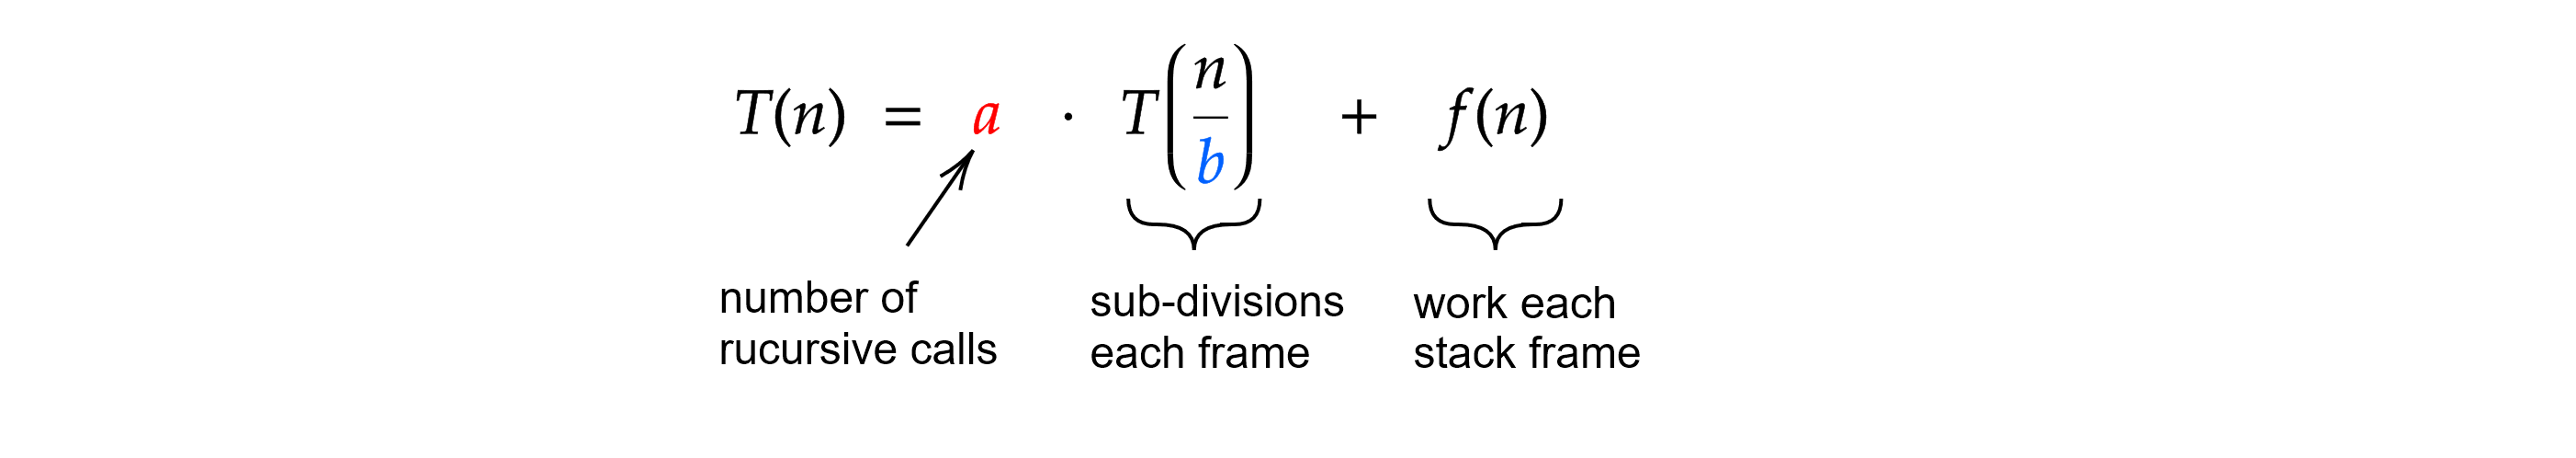
\includegraphics[width=1.2\textwidth]{sections/recurs/rec_form.png}

   
\noindent
For merge sort, we have $T(n) = 2\cdot T(n/2) + \Theta(n)$. This means we i with input $T(n)$ and then 
our first recursive call is $T(n/2)$, the calls from there are $T(n/4)$, $T(n/8)$, and so on. Therefore,
at any given layer $k$, we have $2^k$ calls, with each input $T(n/2^k)$. We stop when $n/2^k = 1$, which is $k = \log n$. Since $2^{\log_2 n} = n$, then $\left(\dfrac{n}{2^{\log_2 n}}\right) = 1$.
Thus, the depth of our recursion is $\log n$, and $n$ work is done when unraveling the stack, hence $O(n \log n)$.

\end{Proof}

\newpage

\noindent
To illustrate the above proof, we can draw a recursion tree for merge sort:\\
\vspace{-5em}
\begin{figure}[h]
    \hspace{-12em}
    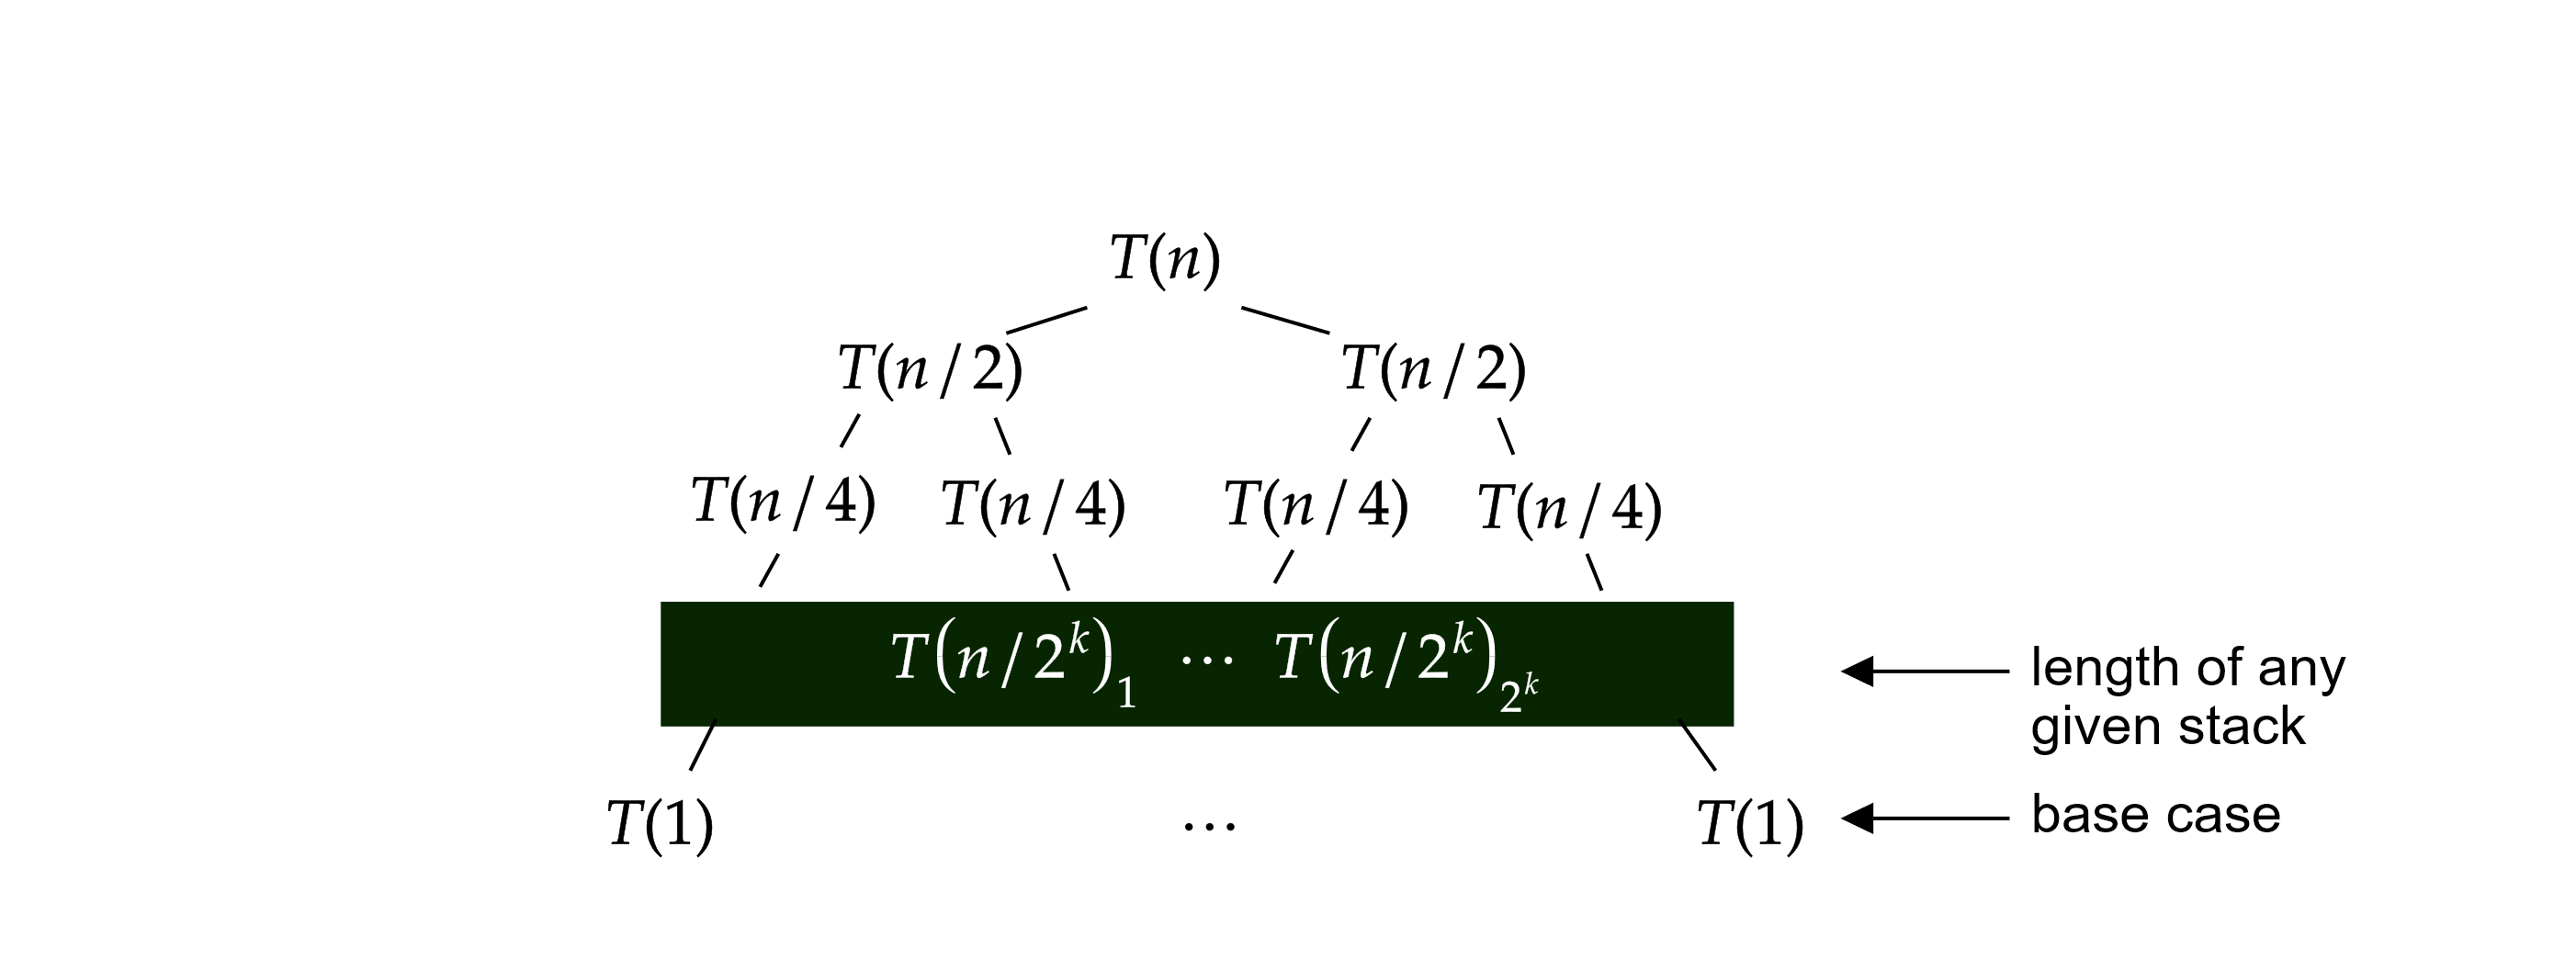
\includegraphics[width=1.5\textwidth]{sections/recurs/rec_tree.png}
    \caption{Recursion Tree for Merge Sort}
\end{figure}

\vspace{-1em}
\begin{Func}[Quicksort - \texttt{QSORT(A)}]
    \textbf{Input:} Array $A$ of $n$ elements.\\
    \textbf{Output:} Sorted array $A$ in ascending order.\\

    \vspace{-.5em}
    \noindent
    \textbf{QSORT function:}\\
    \begin{algorithm}[H]
        \label{algo:quicksort}
        \If{$low < high$}{
            $pivotIndex \gets \texttt{partition}(A, low, high)$\;
            $QSORT(A, low, pivotIndex);$ \tcp{Left of the pivot}
            $QSORT(A, pivotIndex+1, high);$ \tcp{Right of the pivot}
        }
    \end{algorithm}
\end{Func}

\vspace{-1em}
\noindent
\begin{Proof}[Quick Sort - Time Complexity]

    First does $\Theta(n)$ work to partition, then makes 2 recursive calls, and each recursive call 
    has on average $n/2$ elements. We define a general form for our traversals as function $2T(n/2) + \Theta(n)$.
    Thus $\log n$ levels of recursion, each taking $\Theta(n)$ time to partition, hence $O(n \log n)$.\\

    \noindent
    In worst case, $2T(n-1) + \Theta(n)$. Then we have $n$ levels of recursion, each taking $\Theta(n)$ time to partition, hence $O(n^2)$.

\end{Proof}

\newpage

\begin{theo}[Proving Correctness of Recursive Functions]

    To prove correctness of a recursive function, we need to show:
    \begin{enumerate}
        \item \textbf{Base Case:} The base case is correct.
        \item \textbf{Inductive Hypothesis:} Assume $k$ input sizes are correct, where $k<n$, we assume 
        the recursive calls return the correct result.
        \item \textbf{Inductive Step:} Show that the problem reduces to the base case, and that intermediate steps other than the recursive calls are correct.
    \end{enumerate}
    If all three conditions are met, then the function is correct for all $n$.
\end{theo}

\begin{theo}[Master Method for Recursive Time Complexity]

    \label{theo:master}

    The master method is a general technique for solving recurrences of the form:
    \begin{equation*}
        T(n) = \textcolor{red}{a}T\left(\dfrac{n}{\textcolor{blue}{b}}\right) + f(n^{\textcolor{OliveGreen}{d}})
        \end{equation*}
        where $\textcolor{red}{a} \geq 1$, $\textcolor{blue}{b} > 1$, and $f(n)$ is a given function. We consider degree $\textcolor{OliveGreen}{d}$ of $f(n)$:
        \begin{align*}
        \textcolor{OliveGreen}{d} > \log_{\textcolor{blue}{b}} \textcolor{red}{a} &\implies T(n) = \Theta(n^{\textcolor{OliveGreen}{d}}) \\
        \textcolor{OliveGreen}{d} < \log_{\textcolor{blue}{b}} \textcolor{red}{a} &\implies T(n) = \Theta(n^{\log_{\textcolor{blue}{b}} \textcolor{red}{a}}) \\
        \textcolor{OliveGreen}{d} = \log_{\textcolor{blue}{b}} \textcolor{red}{a} &\implies T(n) = \Theta(n^{\log_{\textcolor{blue}{b}} \textcolor{red}{a}} \log n)
        \end{align*}
    
\end{theo}

\begin{Tip}
    Extended Version of the Master Method:
    \\ $$T(n) = f(n) + \sum_{i=1}^{k} a_i T(b_i n + h_i(n))$$
    where  $h_i(n) = O\left( \frac{n}{\log^2 n} \right)$. This is the \textbf{Akra-Bazzi Method}:\\
    Link: \url{https://en.wikipedia.org/wiki/Akra%E2%80%93Bazzi_method}.
\end{Tip}

\textbf{Examples:}
\begin{itemize}
    \item $T(n) = 2T\left(\frac{n}{2}\right) + n^3$: ($a=2$; $b=2$; $d=3$;) then ($\log_2 2 = 1 < 3$) hence $T(n) = \Theta(n^3)$.
    \item $T(n) = 5T\left(\frac{n}{2}\right) + n^2$: ($a=5$; $b=2$; $d=2$;) then ($\log_2 5 \approx 2.32 > 2$) hence $T(n) = \Theta(n^{\log_2 5})$
    \item $T(n) = 16T\left(\frac{n}{4}\right) + n^2$: We have $d:=2$ and ($log_4 16=2=d$) hence $T(n) = \Theta(n^{log_4 16}\log n)$ 
\end{itemize}

\newpage

\begin{Func}[Mergesort - \texttt{MSORT(A)}]
    \textbf{Input:} Array $A$ and temporary array $temp$ of $n$ elements.\\
    \textbf{Output:} Nothing is returned, the array $A$ is sorted by reference.\\

    \vspace{-.5em}
    \noindent
    \textbf{MSORT function:}\\
    \begin{algorithm}[H]
        \label{algo:mergesort}
        \If{$i \geq j$}{
            \Return;
        }
            $mid \gets (i + j) / 2$\;
            $MSORT(A, temp, i, mid);$ \tcp{Left subarray}
            $MSORT(A, temp, mid + 1, j);$ \tcp{Right subarray}
            $merge(A, temp, i, mid, mid + 1, j);$ \tcp{Merge both halves}
        
    \end{algorithm}
\end{Func}

\vspace{-1.5em}
\begin{Proof}[Correctness of Merge Sort]

    By strong induction on the input size $n$:
    
    \begin{enumerate}
        \item \textbf{Base Case:}  
        If $i \geq j$, then the array is of size 1, and is already sorted.
        
        \item \textbf{Inductive Hypothesis:}  
        Assume that Merge Sort correctly sorts arrays of sizes $k$ where $1\leq k < n$.
        
        \item \textbf{Inductive Step:}  
        Our two recursive calls follow, 
        \begin{enumerate}
        \item[(i.)] $mid \gets \floor{(i + j) / 2}$
        \item[(ii.)] $MSORT(A, temp, i, mid)$
        \item[(iii.)] $MSORT(A, temp, mid + 1, j)$
        \end{enumerate}
    \end{enumerate}
    \noindent
    Suppose (ii.) and (iii.) do not reach the base case. Then in (ii.) $mid>=j$ and in (iii.) $mid+1<=i$, which contradicts, as
    $mid:=\floor{(i+j)/2}$, then $i\leq mid \leq j$.\\

    \vspace{-4em}
    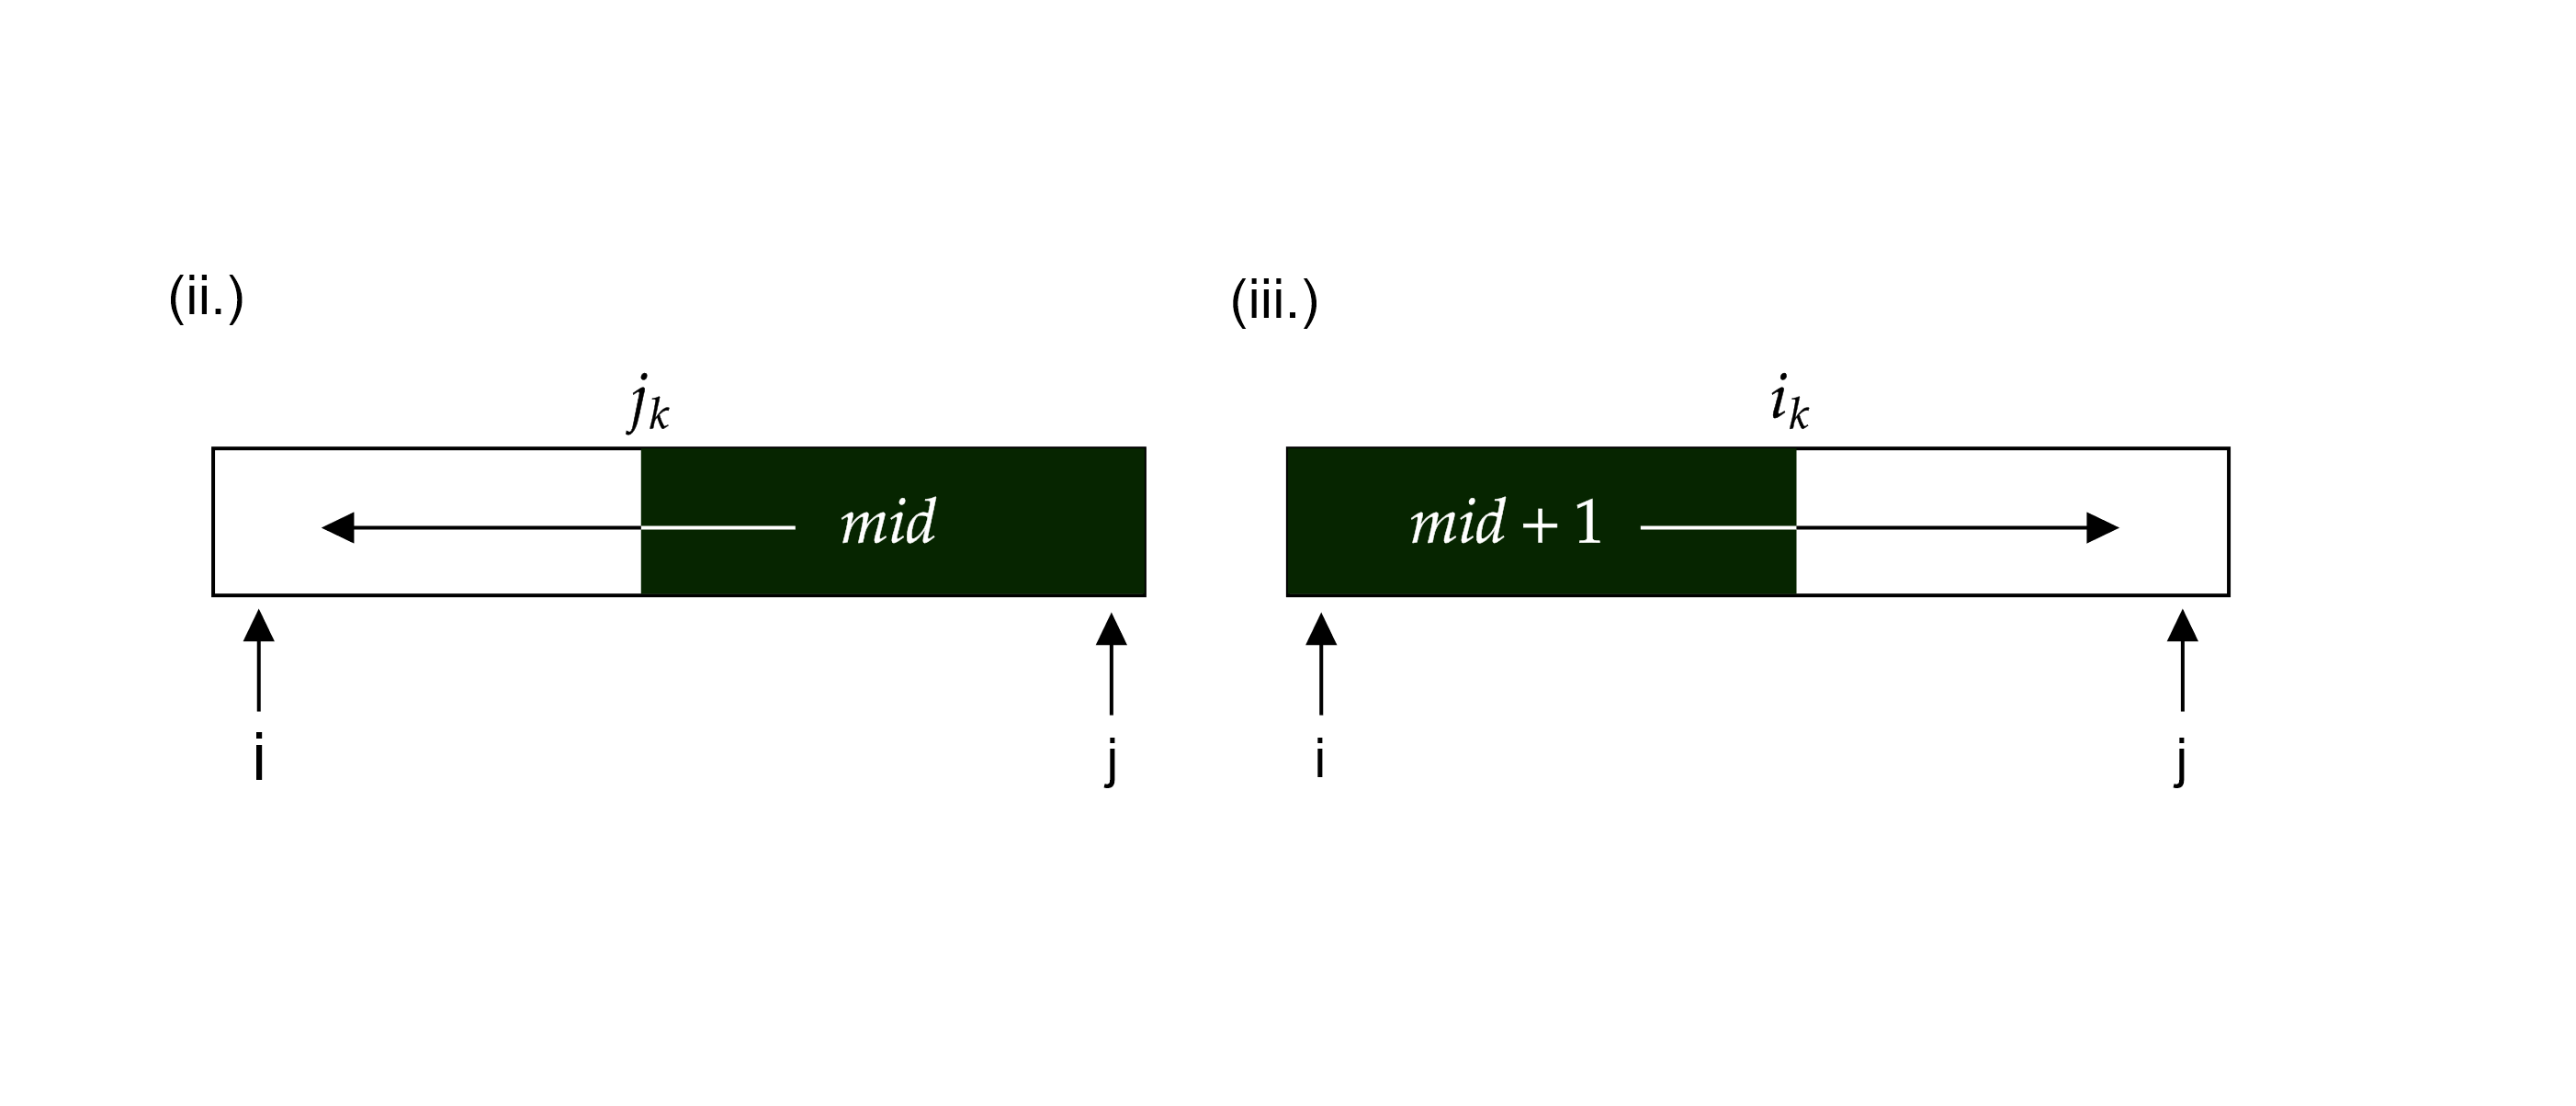
\includegraphics[width=1\textwidth]{sections/recurs/msort_proof.png}

    \vspace{-4em}
    \noindent
    Then in (ii.), the right bound $mid$ keeps decreasing, and in (iii.), the left bound $mid$ keeps increasing.
    This shirks both sub-arrays until both bounds meet. The merge function sorts after both calls, taking the next 
    biggest in the sub-arrays, placing it in the temporary array, and copying back to the original array. Hence, by induction, the function is correct.
\end{Proof}

\newpage

\begin{theo}[Iterative Substitution Method (plug-and-chug)]

    Given a function $T(n)$ which has a recurrence relation---meaning it calls 
    upon itself in its own definition---we may repeatedly substitute such self-references
    back into $T(n)$.

    Given that $T(n)$ properly subdivides to a base case $T(x)$, we may derive some
    pattern which illustrates the state of $T(n)$ at some depth $k$ within the recurrence.
    Doing so, we identify what makes our $k_{th}$ expression hit $T(x)$.
\end{theo}
\begin{Proof}[Iterative Substitution Method (plug-and-chug) - MergeSort]

    Merge sort has the recurrence relation $T(n) = 2T(n/2) + \Theta(n)$, for which the base case is $T(1)$.
    We substitute $T(n/2)$ into $T(n)$:
    \begin{align*}
        T(n) &= 2T(n/2) + \Theta(n);\quad \text{ and }\quad T(n/2) = 2T(n/2^2) + \Theta(n/2);\\
        T(n) &= 2\left[\hspace{3em} \right] + \Theta(n)\text{; Prepare to substitute the recurrence $T(n/2)$}\\
         &= 2\left[2T(n/2^2) + \Theta(n/2)\right] + \Theta(n);\text{ we evaluate $2\cdot\Theta\left(n/2\right)$ as $\Theta\left(2n/2\right)$}\\
         &= 2^2T(n/2^2) + \Theta(n) + \Theta(n)\text{; Simplified}\\
    \end{align*}

    \vspace{-1.5em}
\noindent
We won't fully simplify to observe how the recurrence builds. We continue, evaluating $T(n/2^2)$:
\begin{align*}
    T(n/2^2) &= 2T(n/2^3) + \Theta(n);\\
    T(n) &= 2^2\left[2T(n/2^3) + \Theta(n/2^2)\right] + \Theta(n)+\Theta(n);\text{substitute again}\\
    &= 2^3T(n/2^3) + \Theta(n)+\Theta(n)+\Theta(n)\text{; Simplified}\\
\end{align*}

\vspace{-1.5em}
\noindent
We identify the pattern for the $k_{th}$ substitution:
\begin{align*}
    T(n) &= 2^kT(n/2^k) + k\cdot\Theta(n)\text{; General form}\\
\end{align*}

\vspace{-1.5em}
\noindent
Now we identify what makes our recurrence $T(n/2^k) = T(1)$, i.e., where is $n/2^k = 1$, then $n=2^k$, and $\log_2 n = k$. We plug this back into our general form:
\begin{align*}
    T(n) &= 2^{\log_2 n}T(n/2^{\log_2 n}) + \log_2 n\cdot \Theta(n)\text{; Substituting $k$}\\
    &= n\Theta(1) + \log_2 n\cdot\Theta(n);\text{ Where $T(1)=\Theta(1)$}\\
    &= \Theta(n) + \Theta(n)\log_2 n;\\
    &= \Theta(n\log n);
\end{align*}
Hence, merge sort has a time complexity of $O(n\log n)$.

\end{Proof}

\begin{Tip}
    Live Demo: \url{https://youtu.be/Ob8SM0fz6p0?si=Z4PZQDWOXa7deEHA}
\end{Tip}